	%%%%%%%%%%%%%%%%%%%%%%%%%%%%%%%%%%%%%%%%%%%%%%%%%%%%%%%%%%%%%%%%%%%%%%%%%%%
%%  esrel2025-paper.tex   :   19/12/2018 			                     %%
%%  Text file to use with rps-esrel2023. written in Latex2e.             %%
%%  The content, structure, format and layout of this style file is the  %%
%%  property of Research Publishing Services                             %%
%%  Copyright (c) 2011-2023 Research Publishing Services,                %%
%%  All rights are reserved.                                             %%
%%%%%%%%%%%%%%%%%%%%%%%%%%%%%%%%%%%%%%%%%%%%%%%%%%%%%%%%%%%%%%%%%%%%%%%%%%%

\documentclass[twocolumn]{rps-esrel2026}
%\documentclass[draft, twocolumn]{rps-esrl2026} 

\def\papername{\jobname}

\def\ds{\displaystyle}


%\usepackage[authoryear]{biblatex-chicago}

\usepackage{natbib}
\usepackage{adjustbox}
%\usepackage[authoryear]{natbib}

\begin{document}

\markboth{Temitope Ohiani, Caroline Pyke and Edoardo Patelli}{Information Propagation and Network Analysis in Directed Acyclic Networks: A web interface}

%%%%%%%%%%%%%%%%%%%%%%%%% Plase keep this command for single column for abstract section.
\twocolumn[
%%%%%%%%%%%%%%%%%%%%%%%%%

\title{Information Propagation and Network Analysis in Directed Acyclic Networks: A web interface}

\author{Temitope Ohiani }

\address{Department of Civil and Environmental Engineering, University of Strathclyde, UK. \email{temitope.ohiani@strath.ac.uk}}


\author{Caroline Pyke}

\address{United Kingdom National Nuclear Laboratory, UK. \email{caroline.pyke@uknnl.com}}

\author{Edoardo Patelli}
\address{Department of Civil and Environmental Engineering, University of Strathclyde, UK. \email{edoardo.patelli@strath.ac.uk}}


\begin{abstract}
Domain experts are typically specialists in infrastructure reliability and system analysis, with deep knowledge of their fields. However, they rarely have the time or programming expertise to implement algorithms from scratch. Meanwhile, software developers and computer scientists design, implement, and publish network analysis algorithms. Despite this, a persistent “last mile” gap remains in the adoption of scientific software, driven by barriers to entry and accessibility challenges. This gap becomes even more pronounced when multiple analyses or operating contexts need to be evaluated. Users must often combine multiple tools and algorithms, potentially with different data structures and expectations.

This paper presents a web-based no-code interface for information propagation analysis on directed acyclic networks that addresses this gap. Built on the \texttt{InformationPropagationAnalysis.jl} Julia package, the system offers a fully visual environment for exploring network structures, decomposing subgraphs, performing belief propagation with probability bounds, analyzing capacity, and simulating time and cost propagation. The technology stack separates a Julia computational backend from an Angular browser-based frontend, with both components running entirely on the user's local machine. This design preserves data sovereignty while maintaining flexibility for extension and testing. We demonstrate the software’s features through the WATER wastewater treatment benchmark, evaluating seven operational scenarios spanning both deterministic and interval-typed input data.
\end{abstract}

\keywords{Network Analysis, Information Propagation, Directed Acrylic Networks, System Reliability, Web Interface, Julia.}

%%%%%%%%%%%%%%%%%%%%%%%%% Please keep this closing bracket to complete the single column format for abstract.
]
%%%%%%%%%%%%%%%%%%%%%%%%%

\section{Introduction}

From the design stage to operation and maintenance, decision makers need access to tools and techniques that simultaneously allow them to efficiently model a system's characteristics, as well as trace and quantify the flow of resources against expected metrics. Graph theory has long played a central role in this kind of analysis for civil infrastructures and interconnected systems. The mathematical foundations able to describe the performance of the system and networks and to assess the uncertainty are well established \cite{pearl1988probabilistic, koller2009probabilistic, ferson2013}.  

Unfortunately, it is well known that the people who need these tools most are not always the same ones who develop them. Domain experts often have detailed knowledge of their systems but lack the programming skills required to effectively use many existing software approaches. Sometimes described as the ``last mile problem'', studies consistently report this gap between algorithmic availability and practical adoption~\cite{hannay2009scientists, prabhu2011survey}.

In recent years, several tools have been developed with the goal of making network analysis more accessible, though many of these solutions only address part of the problem. For example, network visualization tools such as Gephi~\cite{bastian2009gephi} and Cytoscape~\cite{shannon2003cytoscape} offer an interactive environment for graph construction and rendering but they do not support any analytical work. These tools usually have to be combined with domain-specific software which often comes with its own data format requirements and a learning curve that can be steep for users that are not familiar with the algorithms.

In many network-based reliability problems, data on component failure rates or link transmission probabilities can be sparse, incomplete, or derived from expert judgement, and require the right tool to fully capture dependency information. Although packages and libraries supporting probabilistic reasoning have been developed for Matlab \cite{OpenCossan}, R~\cite{ferson2019pbar}, Julia~\cite{gray2022pba_julia}, and Python~\cite{gray2022pba}, users wishing to use these methods must be prepared to write code directly against these libraries.

In many cases, no single tool covers both the structural and quantitative aspects of an assessment. Accessibility requirements further reduce the pool of available tools. As a result, complete system profiling often requires combining several of these tools, transforming data between them and managing multiple separate workflows.

Deployment architecture is another important factor that impacts the likelihood of adoption and accessibility of new scientific software. The local-first movement~\cite{kleppmann2019local} encourages the development of software that prioritizes user data sovereignty while maintaining collaborative features. Although cloud-based solutions can be convenient, they raise data sovereignty and privacy concerns~\cite{hashizume2013analysis} that often prevent their use in industries with proprietary data (such as nuclear and defence).

To date, no existing tool offers a fully visual interface that combines structural and quantitative network analysis with native uncertainty quantification while running entirely on the user's local machine. This work addresses this gap by presenting a web-based graphical interface for information propagation analysis on directed acyclic networks. 


\section{The Information Propagation Framework}
As illustrated in Figure~\ref{fig:architecture}, the web interface follows a client-server pattern where both the backend and the frontend run on the user's local machine. This architecture separates the computational backend (developed in Julia) from the interactive browser-based environment written in Angular). This allows each side to be extended, tested, and deployed independently. 

From the end-user's perspective, this separation is invisible; the frontend communicates with the backend through HTTP requests on \texttt{localhost}.

For developers and technical researchers, this already removes the need to reimplement these algorithms from scratch, since the exposed functions can be called directly and the package can be extended or overridden as needed. However, the majority of excluded users are not looking to write code at all.

Domain experts who understand the implications of an analysis and know how to make decisions from results are often not programmers, and these are the users that the web interface was developed for.

\begin{figure*}[t]
    \centering
    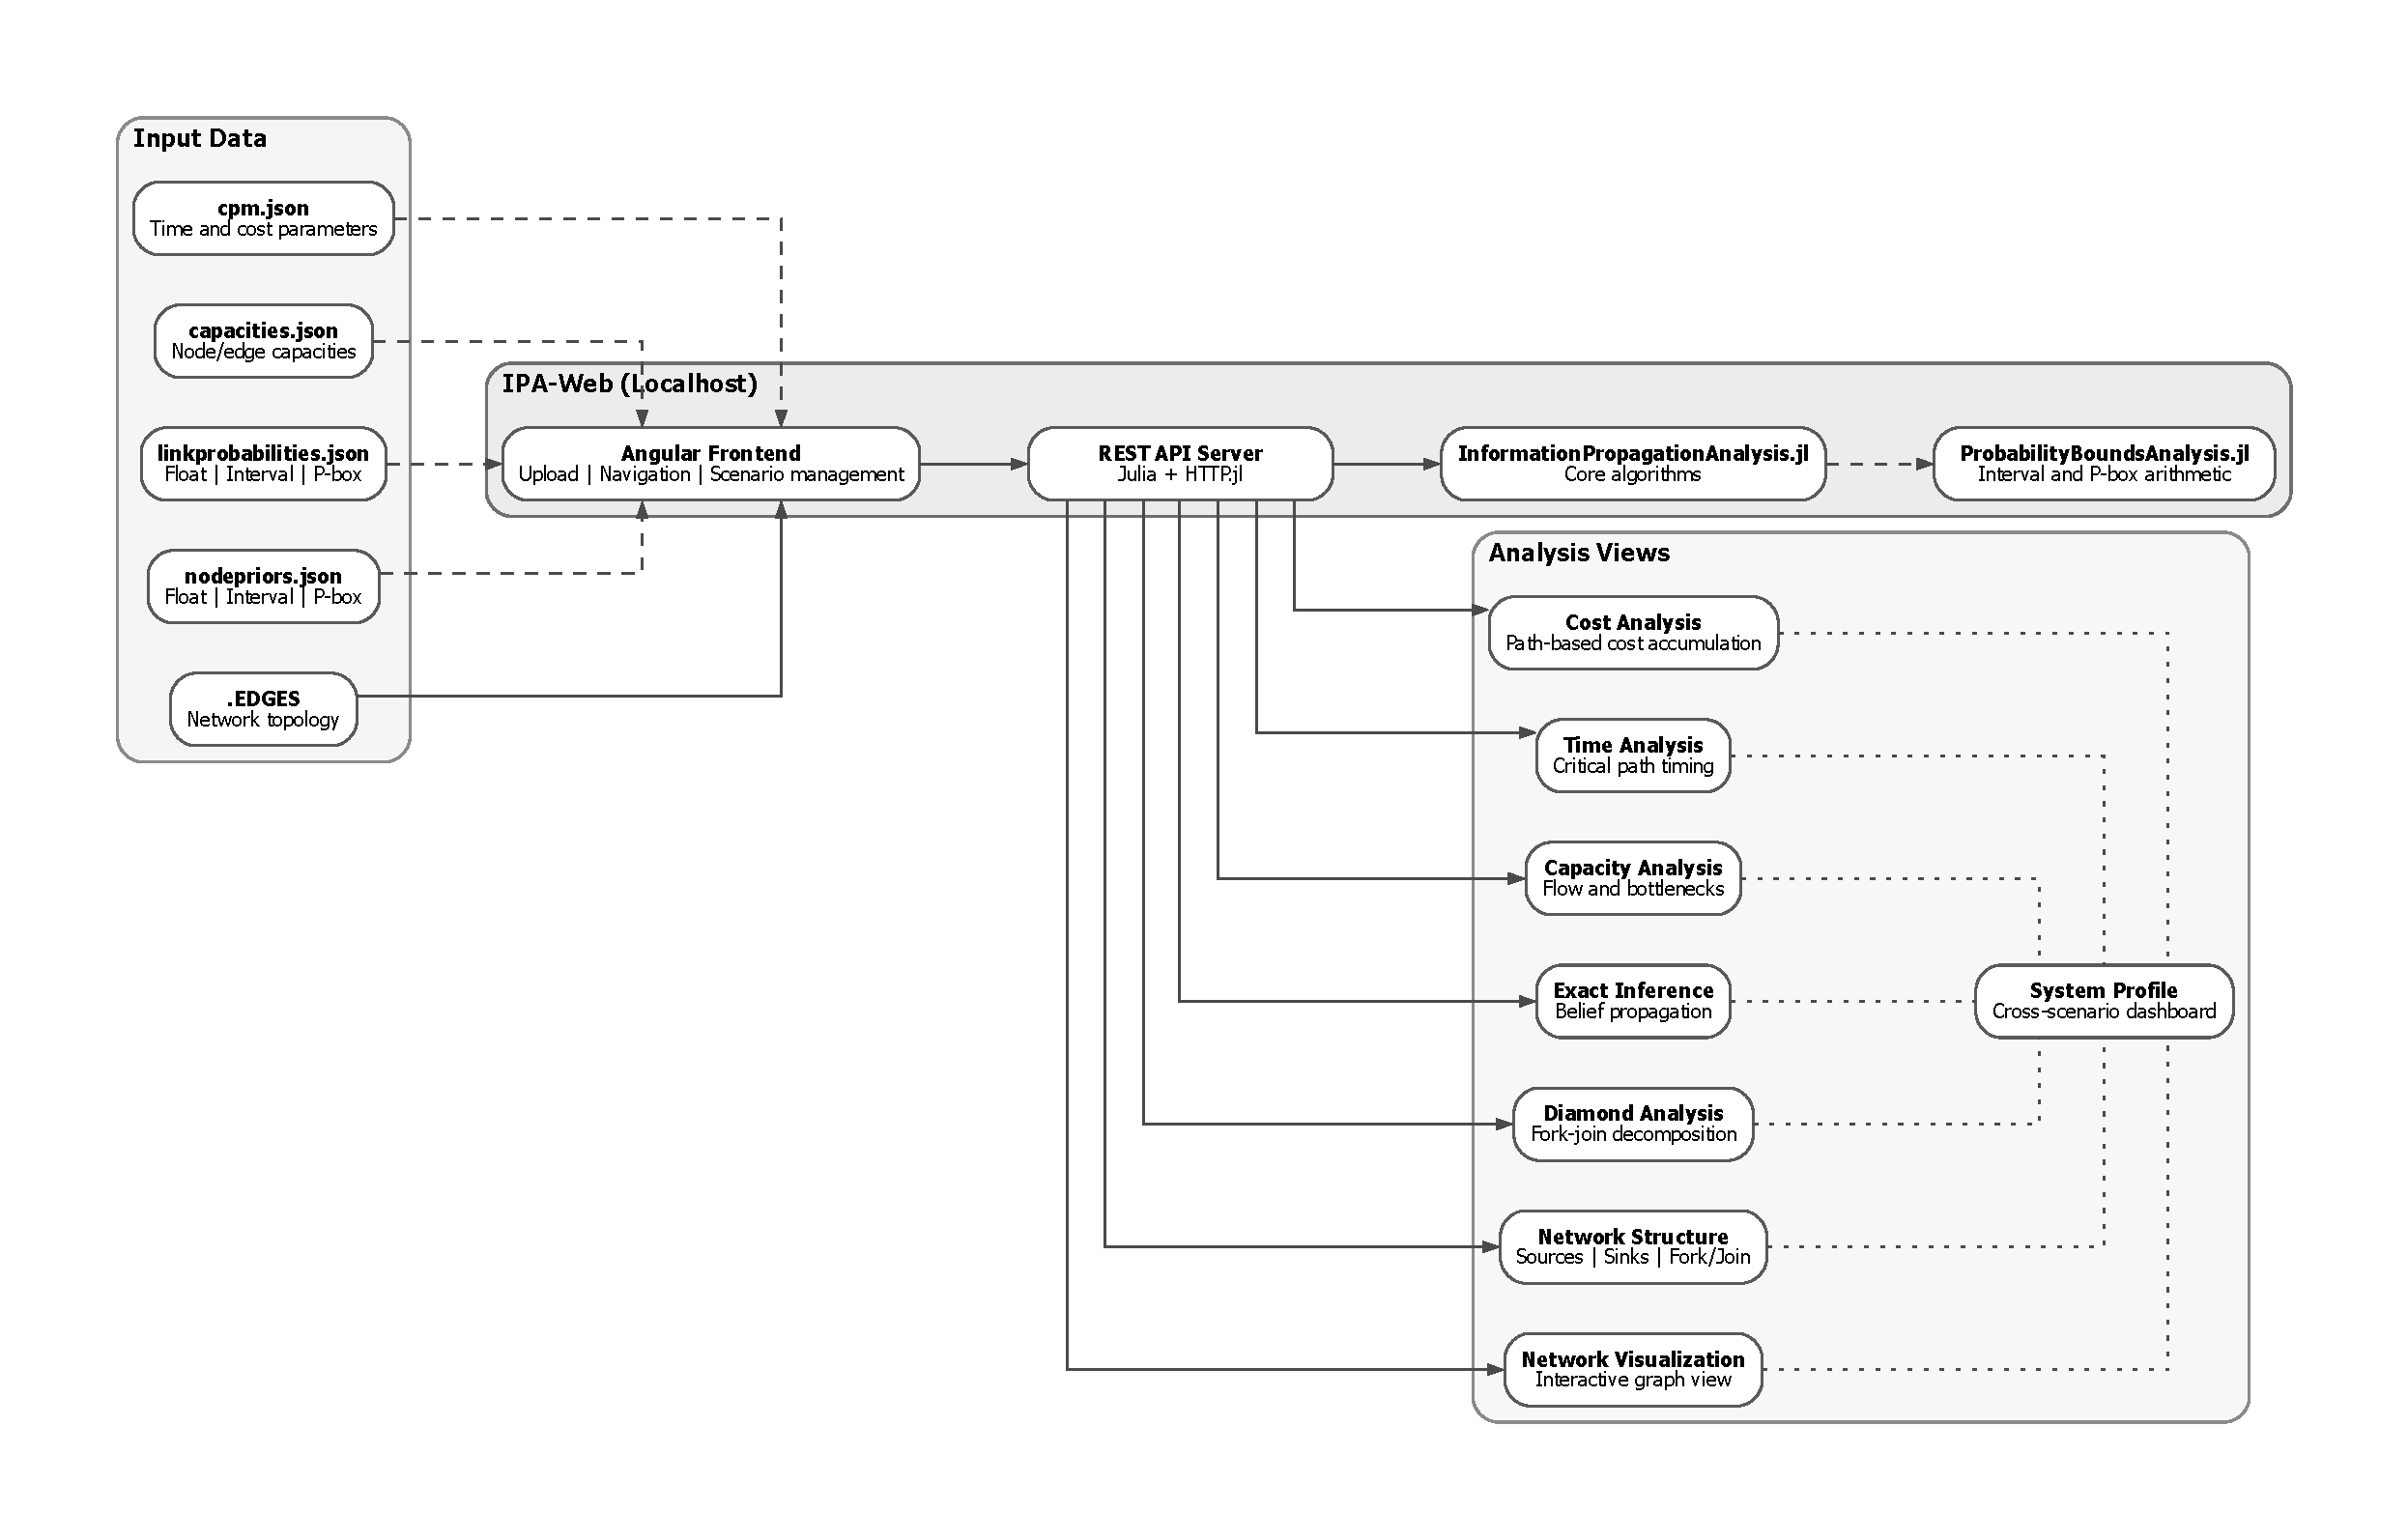
\includegraphics[height=0.45\textheight,width=\textwidth,keepaspectratio]{images/architecture_paper.pdf}
    
    \caption{The IPA-Web decoupled software architecture}
    \label{fig:architecture}
\end{figure*}

\subsection{ Available Network Analysis Tools}
Developed with a Julia language fronte-end and angular backe-end; the \texttt{InformationPropagationAnalysis.jl} package~\cite{infoprop2026_julia} is a multi algorithm framework developed for network analysis in directed acyclic graph (DAG) networks. The framework is made up of five modules. 

The \textbf{Input Processing Module} is the primary entry point into the whole framework. The input module is an I/O handler for parsing and transforming data from raw network files and network adjacency information. Additional network data such as probabilities, cost and time constraints are all handled in this module. For instance, the graph object itself is a structure that contains properties such as adjacency list, precomputed topological sort, ancestor and descendant maps. The result is an enriched graph object (Fig.~\ref{fig:ui_structure_combo}a) that any of the framework's analysis algorithms can query directly with a simple lookup call.

\begin{figure}[t]
    \centering
    
\includegraphics[height=\textheight,width=\linewidth,keepaspectratio]{images/network-visuliation.png}
    
    \vspace{0.5cm}
    
    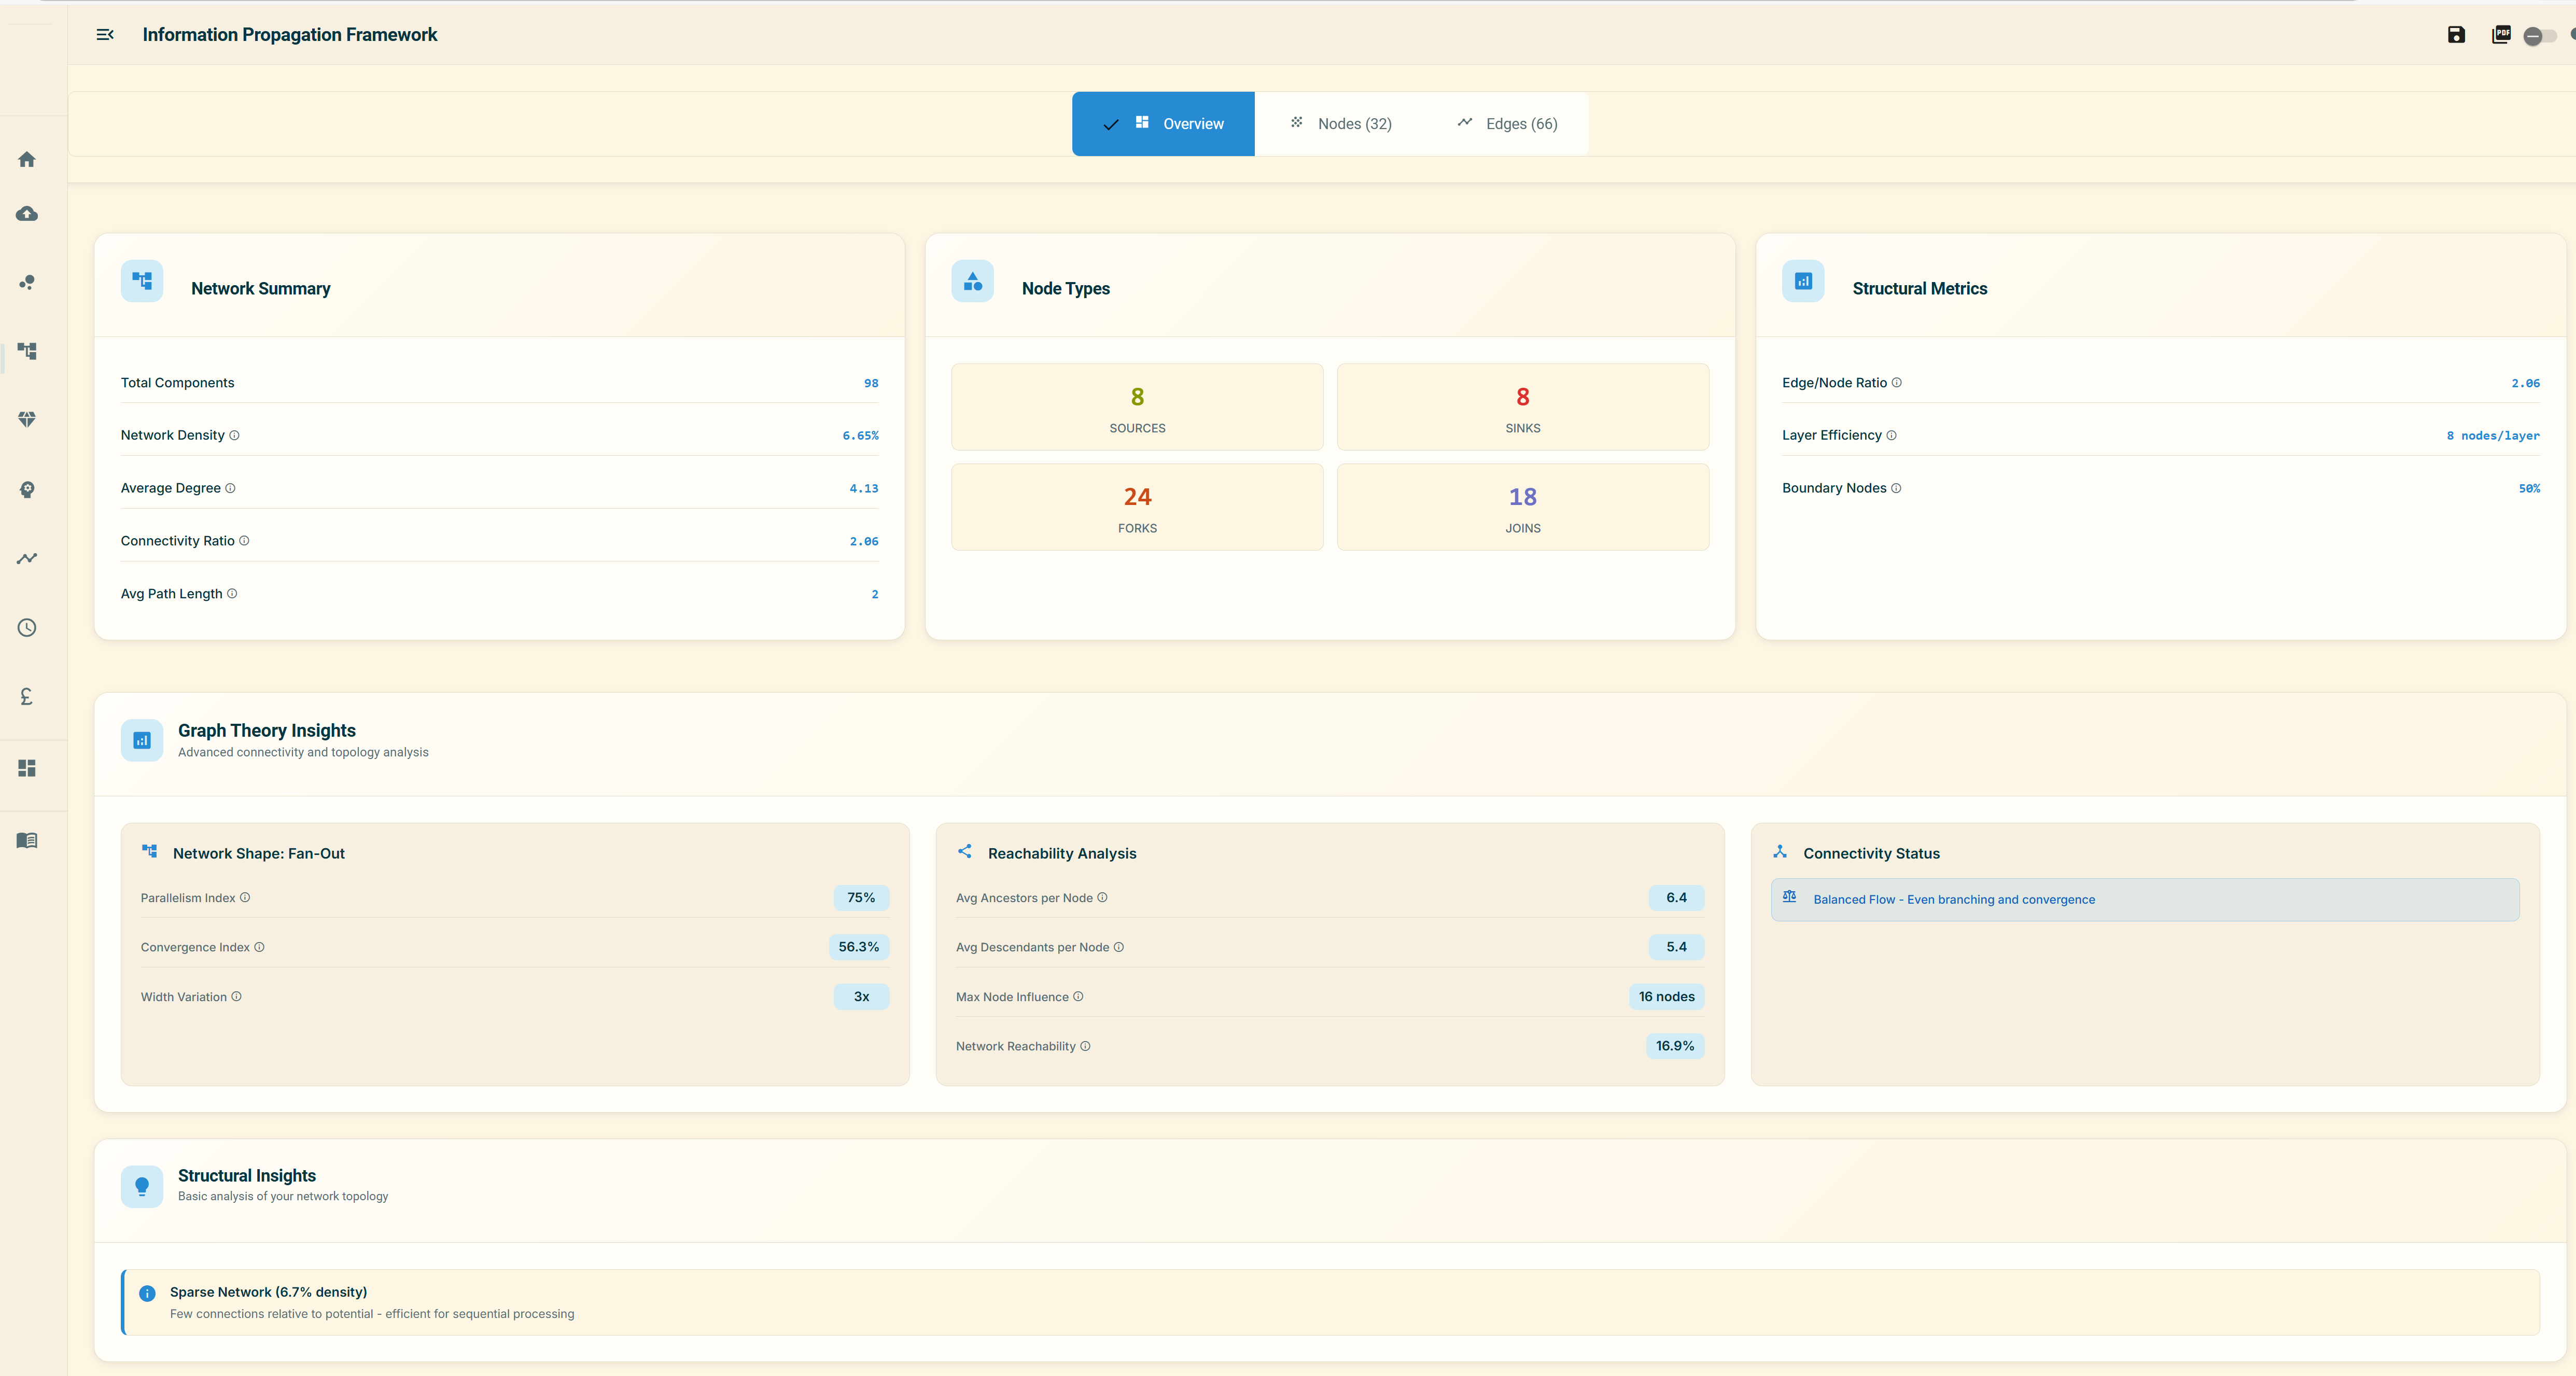
\includegraphics[height=\textheight,width=\linewidth,keepaspectratio]{images/network-structure-view.png}
    
    \caption{Combined graph object view: (a) interactive network visualization and (b) network structure dashboard.}
    \label{fig:ui_structure_combo}
\end{figure}

The \textbf{Subgraph Decomposition Module} scans for and extracts fork-join subgraphs from the enriched graph object. In real infrastructure processes, diamond subgraphs are formed when two or more distinct paths diverge from shared upstream nodes $f_1, \ldots, f_k$ and later re-converge at a downstream join node $j$ that is a descendant of those same shared nodes.

The detection algorithm performs an exhaustive search for all possible diamonds in the network. For optimal traversal, the topological sort from the global graph object drives the discovery order. This order naturally builds a cache of already-discovered diamonds that is drawn on when building and resolving overlapping and nested structures. The sorting ensures that all diamond patterns in the network are processed in a single pass, even when the same previously discovered diamond appears later in the context of a larger diamond.

The advantages of precomputing these subgraphs and their equivalent dependency structures become even more apparent in other modules that employ statistical conditioning and causal reasoning, because the dependency information is already resolved before propagation begins rather than having to be rediscovered and compiled every time a node has diamonds in its ancestry, which in large and dense networks can be costly. Beyond conditional probabilities, the unique diamond objects themselves are stored as the same type of graph object and can therefore be used for isolated or focused evaluation without needing to run a solution on the full network. As with all other modules, the decomposition module is designed to be extendable, so that other subgraph types beyond diamonds can be defined if needed.

The semantic meaning of the node and edge probabilities in the \textbf{Reachability Module} depends on the application context. In a communication network a user might be interested in propagating transmission probabilities, whereas in a reliability model, the same network structure could be used to model component failure rates.  To this end, the module implements an exact belief propagation algorithm that, given the DAG structure, computes at each node the probability that at least one active path reaches it from the source nodes. 
computes at each node the probability that at least one active path reaches it from the source nodes. The belief update at each node $n$ is given by: 
\begin{equation}\label{eq:belief}
B(n) = \pi(n) \cdot P\!\left(\text{at least one working path to } n\right)
\end{equation}
where $\pi(n)$ is the node prior. For a node with parents $p_1, \ldots, p_k$, the ``at least one path'' probability uses inclusion-exclusion:
\begin{equation}\label{eq:inclexcl}
P\!\Bigl(\bigcup_{i=1}^{k} A_i\Bigr) = \sum_{j=1}^{k} (-1)^{j+1} \!\!\sum_{|I|=j} \prod_{i \in I} S_i
\end{equation}
where $S_i = B(p_i) \cdot \ell(p_i, n)$ is the signal through parent $p_i$ and edge probability $\ell(p_i, n)$. For diamond joins, the algorithm conditions on all $2^k$ states of the shared ancestors:
\begin{equation}\label{eq:diamond_cond}
B(j) = \sum_{\mathbf{s} \in \{0,1\}^k} P(\mathbf{s}) \cdot P(j \mid \mathbf{s})
\end{equation}

The message passing sequence follows the topological sort inherited from the input module, and the full algorithmic details are described in detail in ~\cite{infoprop2026} and ~\cite{infoprop2026_julia}. For networks with diamond subgraphs, the causal boundaries through which shared causes must be conditioned can be read directly from those precomputed structures from the decomposition algorithm. Since data quality in real applications is often uneven, by default the BP algorithm supports fixed point values, intervals, and probability boxes (p-boxes) probabilistic data. 
Currently, the module does not support mixed input types within a single run since the input format is expected to match the output format. For mixed probability node and edge information, users may need to standardise their data beforehand. For algorithmic confidence, the module also exposes a full path enumeration method and a Monte Carlo implementation that can be run as independent validation against the algorithm’s results.

Whilst the reachability module answers probabilistic questions about the network, decision makers typically require additional metrics to build a complete system profile. The framework therefore includes two utility modules that extend the probability-based reasoning with capacity and scheduling analysis. In contrast to the belief propagation algorithm, whose cost depends on the number of conditioning nodes in diamond subgraphs (Eq.~\ref{eq:diamond_cond}), both utility modules operate in a single topological pass over the network, requiring $O(|V| + |E|)$ time. For most practical networks, this corresponds to near real-time computation.

The \textbf{Capacity Analysis Module} computes the maximum flow capacity of the network given node capacities, edge capacities, and source input rates. For each non-source node $n$, the sustainable flow is

\begin{equation}\label{eq:maxflow}
F(n) = \min\!\left(\sum_{p \in \mathrm{pa}(n)}
\min\bigl(F(p),\, c_{p \to n}\bigr),\; c_n\right).
\end{equation}

Here $F(p)$ denotes the flow at parent $p$, $c_{p \to n}$ the edge capacity, and $c_n$ the node processing capacity. Beyond maximum flow estimation, the module can identify bottleneck nodes or edges that restrict throughput and determine the widest path, defined as the path whose minimum capacity is maximal from source to target. It also reports overall network throughput as the ratio of total flow reaching target nodes to the total source input rate, providing a direct measure of how effectively the network delivers available input. 

The \textbf{Critical Path Module} serves as a generalized propagation engine where user can decide on the combination function $\bigoplus$,  edge propagation function $f$, and node function $g$. For each non-source node, the resulting value is

\begin{equation}\label{eq:cpm}
V(n) = g\!\left(\bigoplus_{p \in \mathrm{pa}(n)} f\bigl(V(p),\, w_{p \to n}\bigr),\; w_n\right).
\end{equation}

For instance, when $\bigoplus = \max$ and both $f$ and $g$ are additive, Eq.~(\ref{eq:cpm}) reduces to the standard critical path method, and $V(n)$ represents the earliest completion time at node $n$. Setting $\bigoplus = \min$ yields a bottleneck analysis, whereas choosing $\bigoplus = \sum$ produces cost accumulation along paths. Because the module treats these functions as parameters, a single implementation supports multiple analysis types within the same solution.


\section{Application Example: Benchmark Wastewater Treatment Network} 
The user interface is used to evaluate using a well-established benchmark. The WATER network is ~\cite{water_benchmark} is a Bayesian wastewater treatment network commonly used to testing DAG algorithms.  At 32 nodes and 66 directed edges (average Markov blanket size 7.69), it's compact enough to visualize clearly while still exhibiting the structural complexity we want to demonstrate.

More importantly, WATER's internal organization mirrors patterns we often see in real infrastructure systems. It's built from four repeated processing blocks, with dependencies that cross between layers. This creates fork-join patterns at multiple scales, exactly the kind of diamond subgraphs the decomposition module is designed to handle. The layered flow also lets us show how constraints ripple forward through consecutive stages, which is central to capacity analysis in sequential processes. Figure~\ref{fig:ui_structure_combo} shows how users first encounter the network: (a) presents the interactive visual graph object, while (b) summarizes its structural properties once loaded.

\subsection{Scenario design and walkthrough}\label{sec1}
Rather than test the system on a single configuration, seven operation scenarios were developed to  explore different failure modes and  regimes. Five use deterministic inputs to isolate specific bottleneck behaviours: \textit{Edge Bottleneck} restricts transmission capacity while leaving node processing unconstrained; \textit{Node Bottleneck} does the opposite. \textit{Mixed Bottleneck} imposes both types of constraints simultaneously, revealing how they compound. \textit{Source Limited} tests a system where internal capacity is plentiful but input supply falls short. \textit{Single Point of Failure} forces most flow through a critical hub, stressing the network's resilience when redundancy is removed.

The last two scenarios shift from point estimates to interval bounds. \textit{Interval Conservative} applies worst-case parameter values, while \textit{Interval Optimistic} uses best-case bounds. This pairing matters because real reliability assessments rarely have perfect data—operators need to understand not just expected performance but also the range of plausible outcomes under uncertainty.

After running all available analysis including capacity and reachability across all seven scenarios, users can compare results in the System Profile dashboard (Figure~\ref{fig:profile_combo}). The overview panel displays key metrics such as bottleneck locations and critical paths, while the insights panel suggests decision support recommendations, and the optimization panel presents potential improvements. This consolidated view helps operators quickly spot which scenarios produce critical constraints and where interventions might have the greatest impact. The full interface is available on the framework's GitHub page~\cite{infoprop2026_julia}.

\begin{figure*}[p]
    \centering
    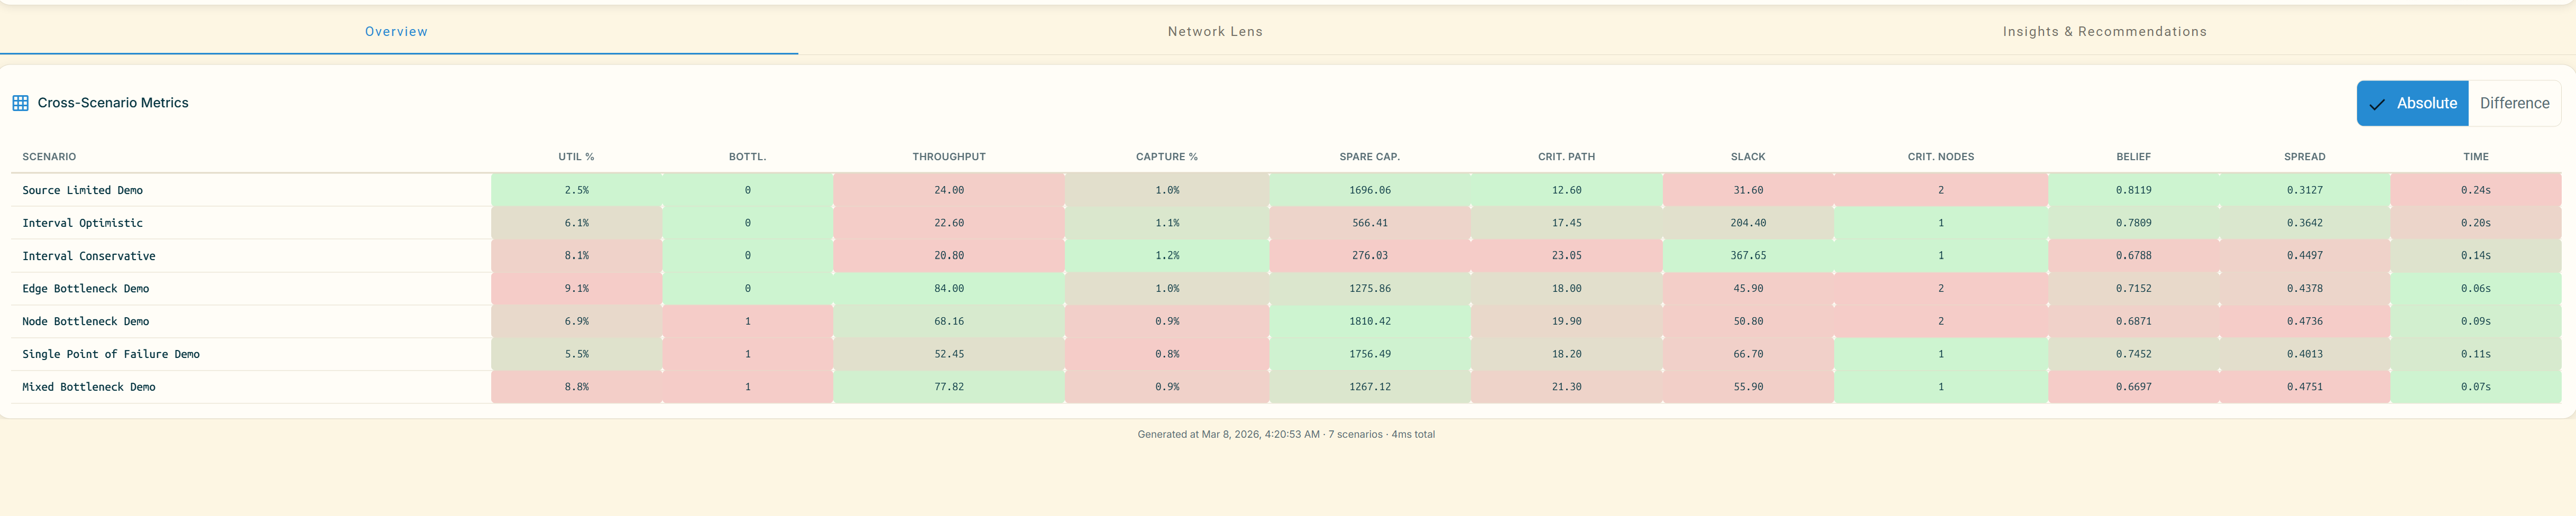
\includegraphics[width=\textwidth,height=0.22\textheight]{images/profile-ovrview.png}
    
    \vspace{0.2em}
    
    
\includegraphics[width=\textwidth,height=0.35\textheight]{images/profile-insights.png}
    
    \vspace{0.2em}
    
    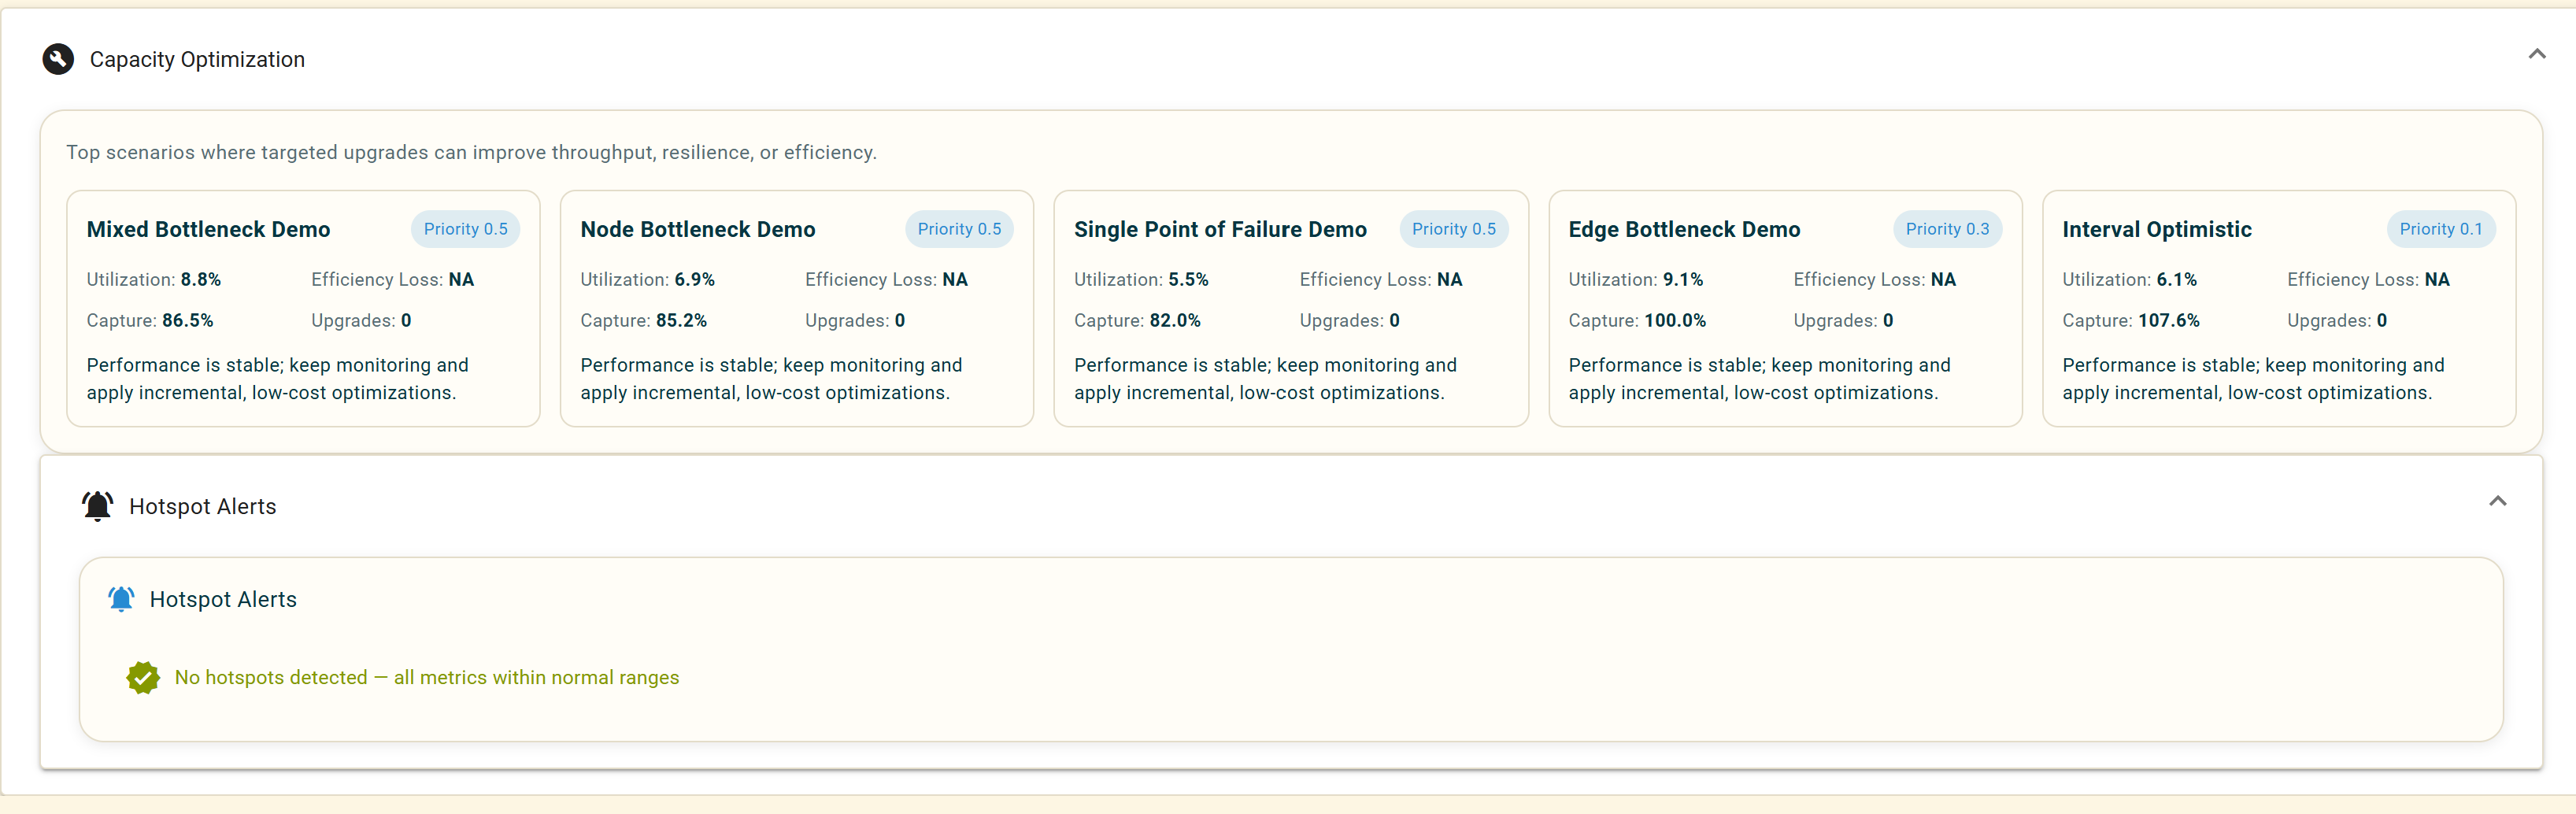
\includegraphics[width=\textwidth,height=0.28\textheight]{images/profile-optimization.png}
    
    \caption{System Profile dashboard: (top) cross-scenario overview, (middle) profile insights for decision support, (bottom) optimization recommendations.}
    \label{fig:profile_combo}
\end{figure*}

\clearpage  
\section{Conclusions}\label{sec:conclusions}

To address the accessibility gap between advanced network analysis algorithms and the domain experts who need them. This paper presents a web-based interactive visual environment for information propagation analysis on directed acyclic networks. 

The proposed software provides a unified full stack toolkit that combines structural analysis, probabilistic reasoning, and resource flow computation within a single workflow. Users can explore network topology, decompose complex fork-join patterns, propagate probabilities with native uncertainty quantification, analyze capacity constraints, and identify critical paths without switching between multiple tools or writing any code. This integration aims to  substantially reduce the cognitive and technical barriers that have historically limited the adoption of these methods in practice.

Beyond visualisation and basic network structure, the framework features multiple propagation and performance analysis modules to allow users to build a complete profile of the system. To reflect the reality of sparse data and expert judgment in real-world reliability assessments, these modules natively support  imprecise probabilistic data through interval and probability boxes. 

By serving both the Julia backend and Angular frontend entirely on the user's machine, the system is designed specifically to guarantee data sovereignty and address privacy concerns that often prevent the use of cloud-based analysis tools with proprietary data. With this decoupled client-server structure, developers and domain experts can independently extend either end of the tech-stack depending on use-case. 

The application of the system to the WATER benchmark network demonstrates its ability to handle realistic infrastructure patterns across multiple operating contexts . The seven scenarios tested span edge-limited, node-limited, and mixed-constraint configurations, as well as interval-valued analyses that bound system performance under parameter uncertainty. The consolidated Profile dashboard shows system performance characteristics results across scenarios, supporting the comparative analysis that target users often need for design decisions.



\begin{acknowledgement}
Temitope Ohiani is supported by the UK National Decommissioning Authority Bursary Studentship "Developing a resilience framework for decommissioning plan of a nuclear facility"


\end{acknowledgement}
\bibliographystyle{chicago}
\bibliography{References}


\end{document}




